% !TEX program = xelatex
\documentclass[a4paper,14pt,oneside,openany]{memoir}

%%% Задаем поля, отступы и межстрочный интервал %%%

\usepackage[left=30mm, right=15mm, top=20mm, bottom=20mm]{geometry}
\pagestyle{plain}
\parindent=1.25cm
\usepackage{indentfirst}

%%% Задаем языковые параметры и шрифт %%%

\usepackage[english,russian]{babel}
\babelfont[russian]{rm}{Times New Roman}
\babelfont[russian]{tt}{Courier New}

%%% Задаем стиль заголовков и подзаголовков в тексте %%%

\setsecnumdepth{subsection}
\renewcommand*{\chapterheadstart}{}
\renewcommand*{\printchaptername}{}
\renewcommand*{\chapnumfont}{\normalfont\bfseries}
\renewcommand*{\afterchapternum}{\hspace{1em}}
\renewcommand*{\printchaptertitle}{\normalfont\bfseries\centering\MakeUppercase}
\setbeforesecskip{20pt}
\setaftersecskip{20pt}
\setsecheadstyle{\raggedright\normalfont\bfseries}
\setbeforesubsecskip{20pt}
\setaftersubsecskip{20pt}
\setsubsecheadstyle{\raggedright\normalfont\bfseries}

%%% Исправление нумерации секций %%%

\renewcommand{\thesection}{\arabic{section}}
\renewcommand{\thesubsection}{\arabic{subsection}}

%%% Сквозная нумерация рисунков и таблиц %%%

\counterwithout{figure}{chapter}
\counterwithout{table}{chapter}

%%% Выравнивание и переносы %%%

\tolerance 1414
\hbadness 1414
\emergencystretch 1.5em
\clubpenalty=10000
\widowpenalty=10000

%%% Задаем параметры оформления рисунков и таблиц %%%

\usepackage{graphicx}
\usepackage{caption}
\usepackage{subcaption}
\usepackage{float}
\graphicspath{{photo/}}
\captionsetup[figure]{font=small, width=\textwidth, name=Рисунок, justification=centering}
\captiondelim{ --- }
\usepackage[section]{placeins}

%%% Задаем параметры ссылок и гиперссылок %%% 

\usepackage{hyperref}
\hypersetup{
    colorlinks=true,
    linkcolor=red,
    citecolor=red
}

%%% Настраиваем отображение списков %%%

\usepackage{enumitem}
\renewcommand*{\labelitemi}{\normalfont{--}}
\setlist{noitemsep, leftmargin=*}

\begin{document}

% Титульный лист (без номера страницы)
\thispagestyle{empty}

\begin{center}
    МИНИСТЕРСТВО ЦИФРОВОГО РАЗВИТИЯ, СВЯЗИ И МАССОВЫХ \\ КОММУНИКАЦИЙ \\ РОССИЙСКОЙ ФЕДЕРАЦИИ

    \vspace{20pt}

    Федеральное государственное бюджетное образовательное учреждение \\ высшего образования \\
    "Сибирский государственный университет телекоммуникаций и \\ информатики"

    \vspace{20pt}

    Кафедра телекоммуникационных систем и вычислительных средств \\ (ТС и ВС)
\end{center}

\vfill

\begin{center}
    Практическая работа №8 \\
    по дисциплине \\
    \textit{"Web-технологии"}

    \vspace{20pt}

    по теме: \\
    \uppercase{Установка и настройка системы управления контентом WordPress. Настройка PrivateBin}
\end{center}

\vfill

\noindent Студент: \\
\textit{Группа ИКС-532 \hfill А.С. Лёшин}

\vspace{20pt}

\noindent Преподаватель: \\
\textit{старший преподаватель \hfill А.В. Андреев}

\vfill

\begin{center}
    Новосибирск 2026 г.
\end{center}

\newpage
\setcounter{page}{2}
\OnehalfSpacing*

\subsection*{Цель работы}

\begin{itemize}
    \item Установка и настройка системы управления контентом WordPress на базе LAMP.
    \item Развёртывание сервиса PrivateBin для безопасной передачи паролей.
    \item Обеспечение взаимодействия PrivateBin с почтовым сервером iRedMail (лабораторная работа №7).
\end{itemize}

\section{WordPress: Подготовка инфраструктуры}

Первым этапом настройки является конфигурация статического IP-адреса. На \hyperref[fig-wpip]{рисунке \ref*{fig-wpip}} представлено содержимое файла \texttt{/etc/netplan/00-installer-config.yaml} после редактирования.

\begin{figure}[H]
    \centering
    
\includegraphics[width=0.6\textwidth]{photo/photo1.png}
    \caption{Содержимое файла /etc/netplan/00-installer-config.yaml}
    \label{fig-wpip}
\end{figure}

Проверить правильность настройки можно командой \texttt{ip a} и проверкой доступа в интернет командой \texttt{ping ya.ru}. На \hyperref[fig-wpipa]{рисунке \ref*{fig-wpipa}} представлен вывод команды.

\begin{figure}[H]
    \centering
    
\includegraphics[width=0.6\textwidth]{photo/photo2.png}
    \caption{Вывод команды ip a }
    \label{fig-wpipa}
\end{figure}

\section{WordPress: Настройка DNS}

Для корректной работы сервера необходимо добавить прямую и обратную записи в DNS на сервере Gateway. На \hyperref[fig-wp-forward]{рисунке \ref*{fig-wp-forward}} показан процесс добавления прямой записи в домен, а на \hyperref[fig-wp-reverse]{рисунке \ref*{fig-wp-reverse}} — обратной записи.

\begin{figure}[H]
    \centering
    
\includegraphics[width=0.8\textwidth]{photo/photo3.png}
    \caption{Добавление прямой записи для WordPress в DNS}
    \label{fig-wp-forward}
\end{figure}

\begin{figure}[H]
    \centering
    
\includegraphics[width=0.8\textwidth]{photo/photo4.png}
    \caption{Добавление обратной записи для WordPress в DNS}
    \label{fig-wp-reverse}
\end{figure}

После добавления записей выполняется проверка работоспособности DNS. На \hyperref[fig-wp-dns-check]{рисунке \ref*{fig-wp-dns-check}} представлен результат проверки с помощью \texttt{nslookup} и \texttt{ping}.

\begin{figure}[H]
    \centering
    
\includegraphics[width=0.6\textwidth]{photo/photo5.png}
    \caption{Проверка работы DNS для WordPress (nslookup и ping)}
    \label{fig-wp-dns-check}
\end{figure}

\section{WordPress: Установка LAMP и настройка}

Устанавливается LAMP (Linux-Apache-MySQL-PHP) сервер. После установки в файл \texttt{/etc/apache2/apache2.conf} добавляется директива \texttt{ServerName localhost} (на \hyperref[fig-wp-apache]{рисунке \ref*{fig-wp-apache}}).

\begin{figure}[H]
    \centering
    
\includegraphics[width=0.6\textwidth]{photo/photo6.png}
    \caption{Редактирование файла /etc/apache2/apache2.conf}
    \label{fig-wp-apache}
\end{figure}

Далее изменяются права на содержимое каталога \texttt{/var/www} (на \hyperref[fig-wp-chown]{рисунке \ref*{fig-wp-chown}}).

\begin{figure}[H]
    \centering
    
\includegraphics[width=0.6\textwidth]{photo/photo7.png}
    \caption{Изменение прав на каталог /var/www}
    \label{fig-wp-chown}
\end{figure}

На \hyperref[fig-wp-config-edit]{рисунке \ref*{fig-wp-config-edit}} показан процесс редактирования файла \texttt{wp-config.php}, где указываются параметры подключения к базе данных.

\begin{figure}[H]
    \centering
    
\includegraphics[width=0.8\textwidth]{photo/photo8.png}
    \caption{Редактирование wp-config.php}
    \label{fig-wp-config-edit}
\end{figure}

После настройки файлы WordPress копируются в корень документа Apache, а установка завершается через веб-интерфейс.

\section{WordPress: Завершение установки через веб-интерфейс}

Переходим по адресу \texttt{http://wordpress.leshin.X-532.local}. На \hyperref[fig-wp-login]{рисунке \ref*{fig-wp-login}} показана страница входа в панель администратора после завершения установки.

\begin{figure}[H]
    \centering
    
\includegraphics[width=0.8\textwidth]{photo/photo9.png}
    \caption{Страница входа в панель администратора WordPress}
    \label{fig-wp-login}
\end{figure}

Далее создаются тестовые записи в блоге. На \hyperref[fig-wp-post1]{рисунке \ref*{fig-wp-post1}} и \hyperref[fig-wp-post2]{рисунке \ref*{fig-wp-post2}} показан процесс добавления новых записей.

\begin{figure}[H]
    \centering
    
\includegraphics[width=0.8\textwidth]{photo/photo10.png}
    \caption{Создание новой записи в WordPress}
    \label{fig-wp-post1}
\end{figure}

\begin{figure}[H]
    \centering
    
\includegraphics[width=0.8\textwidth]{photo/photo11.png}
    \caption{Создание второй записи в WordPress}
    \label{fig-wp-post2}
\end{figure}

На \hyperref[fig-wp-main]{рисунке \ref*{fig-wp-main}} представлен вид главной страницы сайта с опубликованными записями.

\begin{figure}[H]
    \centering
    
\includegraphics[width=0.8\textwidth]{photo/photo12.png}
    \caption{Главная страница WordPress с опубликованными записями}
    \label{fig-wp-main}
\end{figure}

\section{PrivateBin: Подготовка инфраструктуры}

Первым этапом настройки PrivateBin является конфигурация статического IP-адреса. На \hyperref[fig-pb-ip]{рисунке \ref*{fig-pb-ip}} представлено содержимое файла \texttt{/etc/netplan/00-installer-config.yaml} после редактирования.

\begin{figure}[H]
    \centering
    
\includegraphics[width=0.6\textwidth]{photo/photo13.png}
    \caption{Содержимое файла /etc/netplan/00-installer-config.yaml}
    \label{fig-pb-ip}
\end{figure}

Проверить правильность настройки можно командой \texttt{ip a}. На \hyperref[fig-pb-ipa]{рисунке \ref*{fig-pb-ipa}} представлен вывод команды.

\begin{figure}[H]
    \centering
    
\includegraphics[width=0.6\textwidth]{photo/photo14.png}
    \caption{Вывод команды ip a }
    \label{fig-pb-ipa}
\end{figure}

\section{PrivateBin: Настройка DNS}

Для корректной работы PrivateBin необходимо добавить прямую и обратную записи в DNS на сервере Gateway. На \hyperref[fig-pb-forward]{рисунке \ref*{fig-pb-forward}} показан процесс добавления прямой записи в домен, а на \hyperref[fig-pb-reverse]{рисунке \ref*{fig-pb-reverse}} — обратной записи.

\begin{figure}[H]
    \centering
    
\includegraphics[width=0.8\textwidth]{photo/photo15.png}
    \caption{Добавление прямой записи для PrivateBin в DNS}
    \label{fig-pb-forward}
\end{figure}

\begin{figure}[H]
    \centering
    
\includegraphics[width=0.8\textwidth]{photo/photo16.png}
    \caption{Добавление обратной записи для PrivateBin в DNS}
    \label{fig-pb-reverse}
\end{figure}

После добавления записей выполняется проверка работоспособности DNS. На \hyperref[fig-pb-dns-check]{рисунке \ref*{fig-pb-dns-check}} представлен результат проверки.

\begin{figure}[H]
    \centering
    
\includegraphics[width=0.6\textwidth]{photo/photo17.png}
    \caption{Проверка работы DNS для PrivateBin (nslookup и ping)}
    \label{fig-pb-dns-check}
\end{figure}

\section{PrivateBin: Настройка Apache и SSL}

Для работы PrivateBin по протоколу HTTPS создаётся конфигурационный файл виртуального хоста. На \hyperref[fig-pb-apache-conf]{рисунке \ref*{fig-pb-apache-conf}} показано содержимое файла \texttt{/etc/apache2/sites-available/privatebin.conf}.

\begin{figure}[H]
    \centering
    
\includegraphics[width=0.6\textwidth]{photo/photo18.png}
    \caption{Конфигурация виртуального хоста для PrivateBin}
    \label{fig-pb-apache-conf}
\end{figure}

\section{PrivateBin: Проверка работы и взаимодействие с почтовым сервером}

После настройки веб-сервер PrivateBin доступен по адресу \texttt{https://privatebin.leshin.X-532.local}. На \hyperref[fig-pb-main]{рисунке \ref*{fig-pb-main}} представлена главная страница сервиса.

\begin{figure}[H]
    \centering
    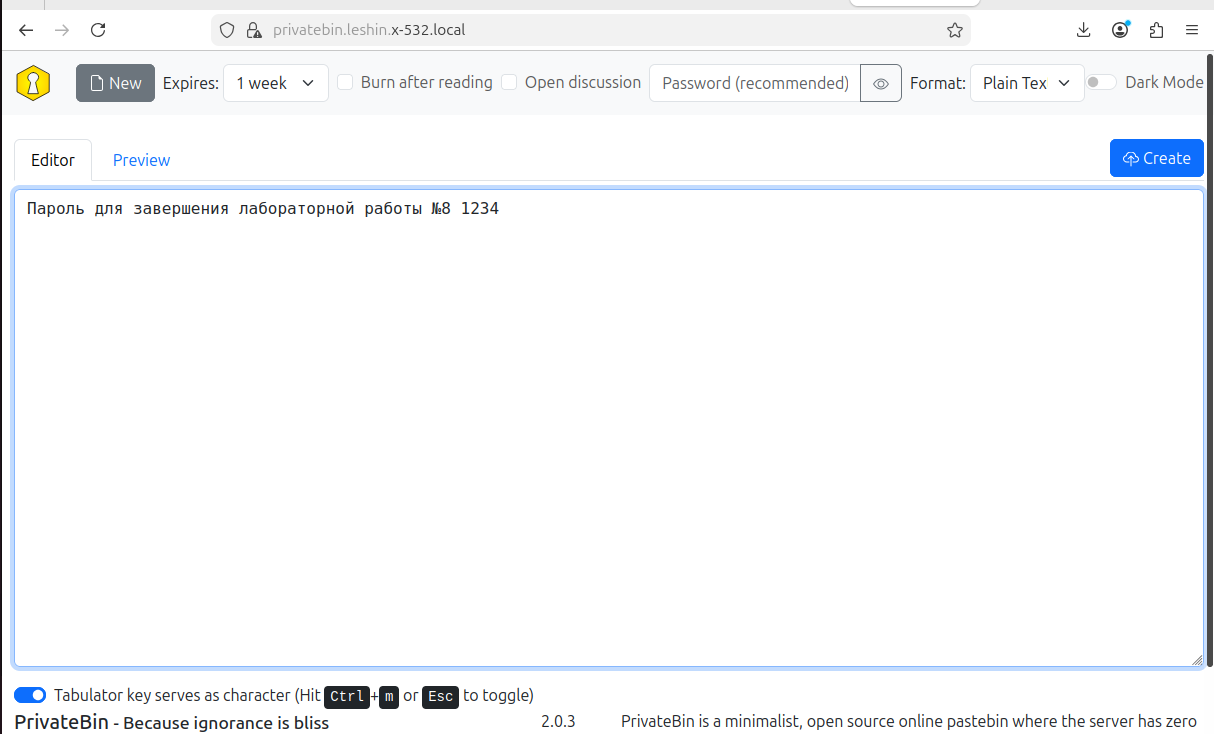
\includegraphics[width=0.6\textwidth]{photo/photo19.png}
    \caption{Главная страница PrivateBin}
    \label{fig-pb-main}
\end{figure}

На \hyperref[fig-pb-paste]{рисунке \ref*{fig-pb-paste}} показана созданная запись в PrivateBin.

\begin{figure}[H]
    \centering
    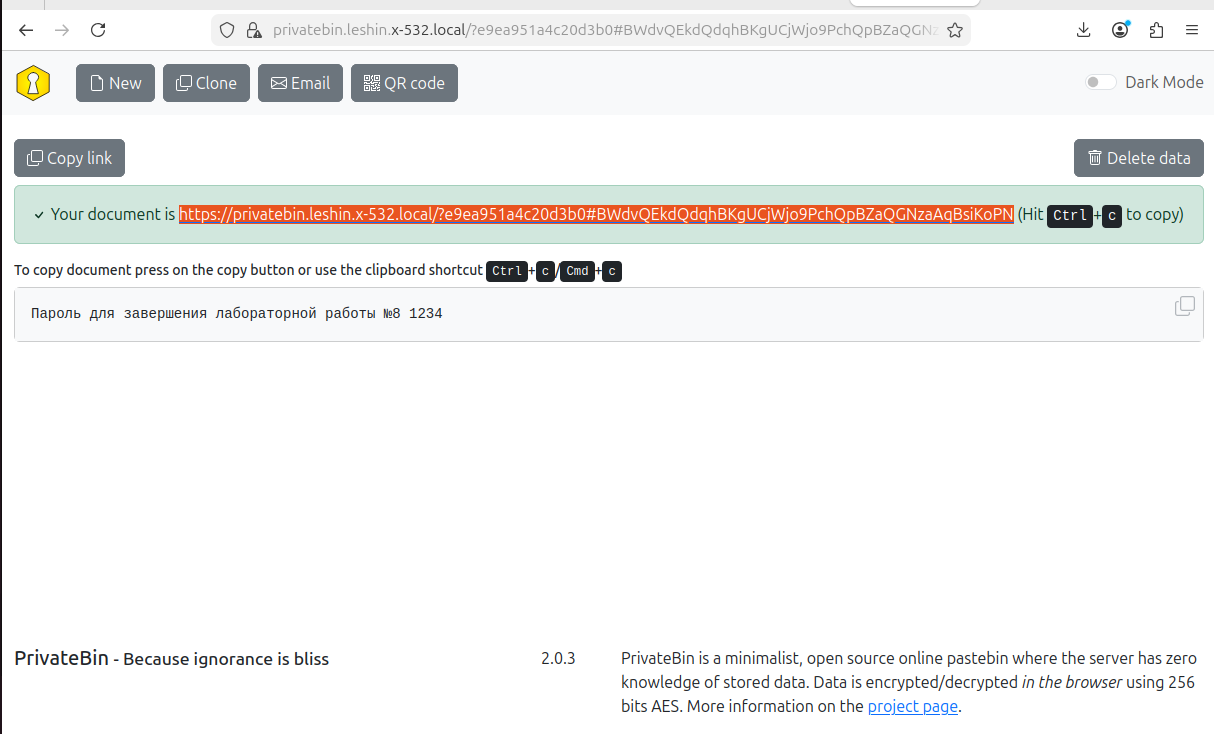
\includegraphics[width=0.8\textwidth]{photo/photo20.png}
    \caption{Создание записи с паролем в PrivateBin}
    \label{fig-pb-paste}
\end{figure}

Ссылка на запись отправляется с почтового ящика \texttt{user1} на \texttt{postmaster}. На \hyperref[fig-pb-email-send]{рисунке \ref*{fig-pb-email-send}} показано отправленное письмо.

\begin{figure}[H]
    \centering
    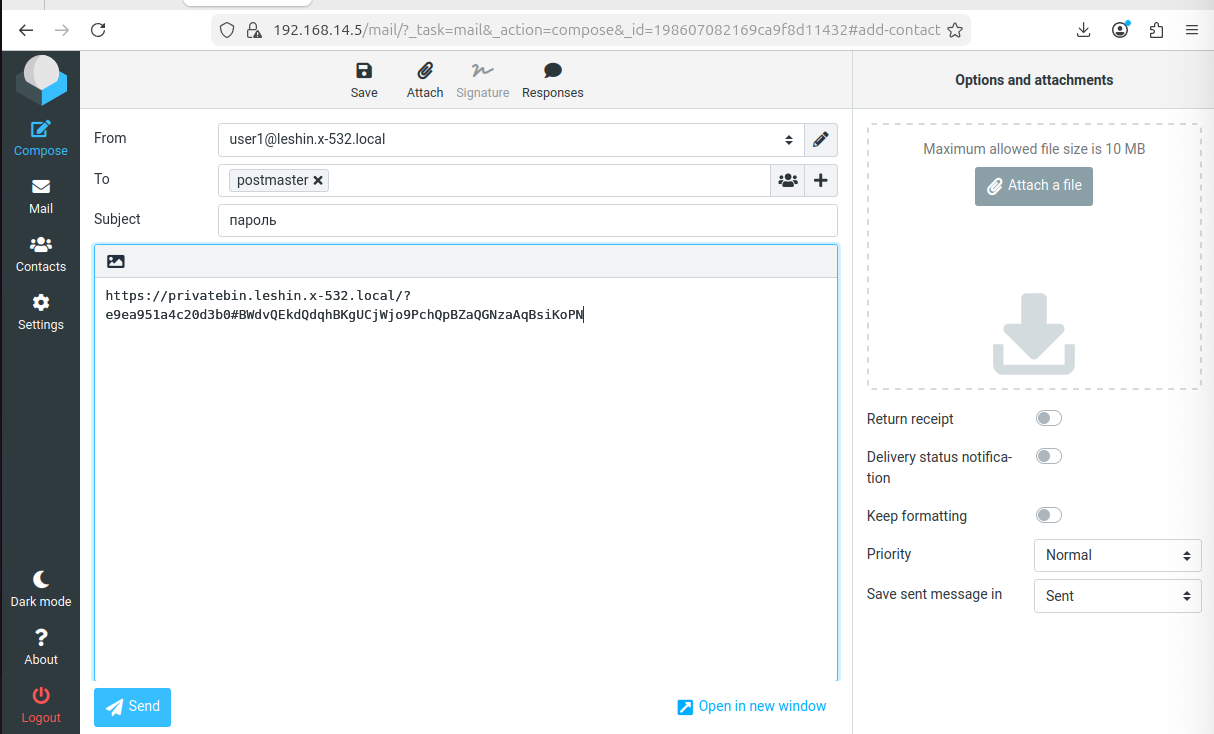
\includegraphics[width=0.8\textwidth]{photo/photo21.png}
    \caption{Отправка ссылки на пароль по электронной почте}
    \label{fig-pb-email-send}
\end{figure}

На \hyperref[fig-pb-email-received]{рисунке \ref*{fig-pb-email-received}} представлено полученное письмо в ящике \texttt{postmaster}.

\begin{figure}[H]
    \centering
    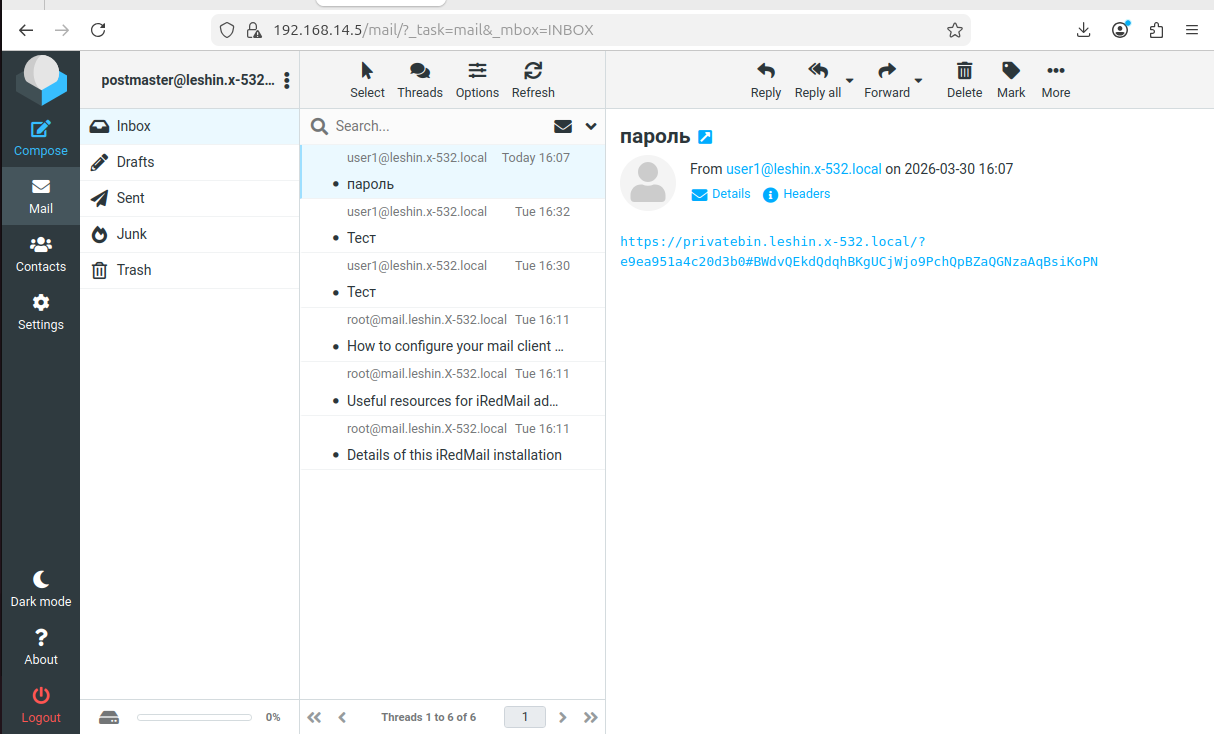
\includegraphics[width=0.8\textwidth]{photo/photo22.png}
    \caption{Полученное письмо со ссылкой на пароль}
    \label{fig-pb-email-received}
\end{figure}

После перехода по ссылке открывается страница с сохранённым паролем, что подтверждает успешное выполнение задания (\hyperref[fig-pb-password]{рисунок \ref*{fig-pb-password}}).

\begin{figure}[H]
    \centering
    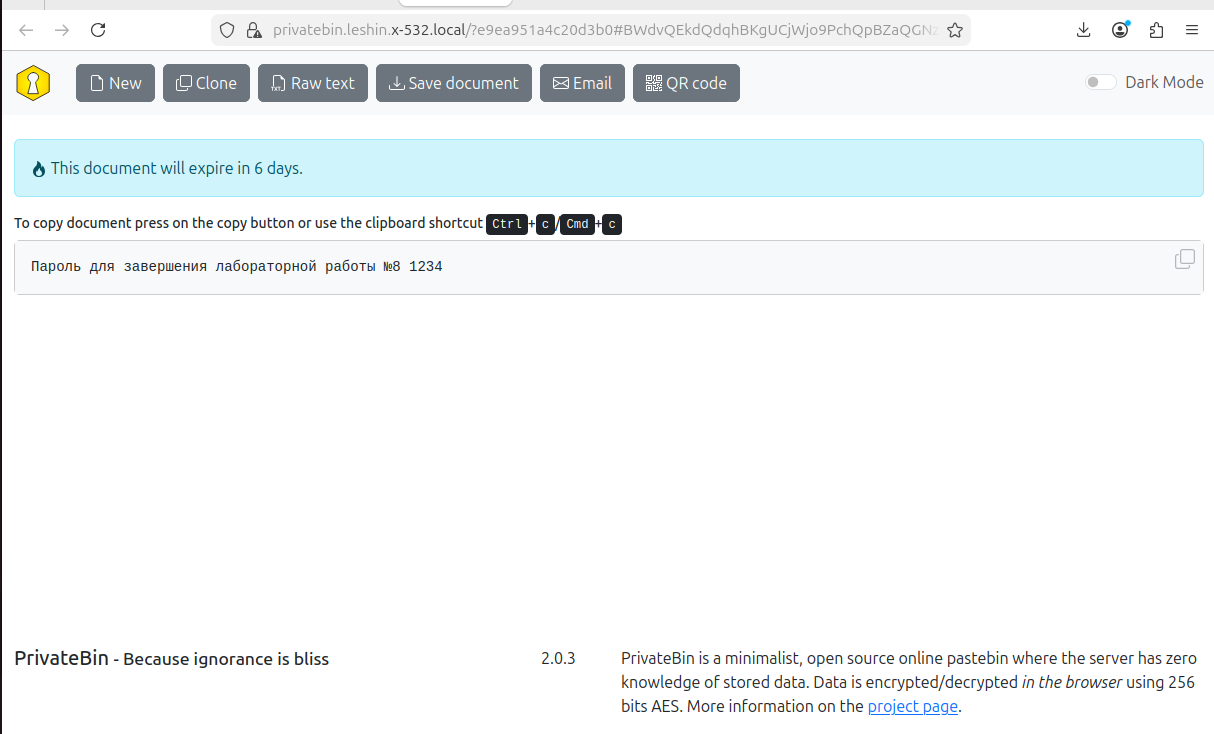
\includegraphics[width=0.8\textwidth]{photo/photo23.png}
    \caption{Страница PrivateBin с сохранённым паролем}
    \label{fig-pb-password}
\end{figure}

\section*{Заключение}
\addcontentsline{toc}{section}{Заключение}

В ходе выполнения работы были решены следующие задачи:
\begin{enumerate}
    \item Развёрнута система управления контентом WordPress на основе LAMP-стека.
    \item Настроен DNS-сервер для обеспечения доступа к сайту по имени \texttt{wordpress.leshin.X-532.local}.
    \item Созданы тестовые записи в блоге, подтверждающие работоспособность сайта.
    \item Установлен и настроен сервис PrivateBin для безопасной передачи паролей.
    \item Обеспечено взаимодействие PrivateBin с почтовым сервером iRedMail: ссылка на пароль успешно передана по электронной почте.
\end{enumerate}

\end{document}